% !Mode:: "TeX:UTF-8"

\chapter{SpringBoot项目}
\section{项目需求}
本项目主要使用VUE+SpringBoot+AJAX技术,开发前后端分离的Web应用程序。由于本项目中的前端VUE代码和数据库结构与第三阶段Servlet项目一致,且项目需求与第三阶段一致,只是将服务器端代码由Servlet升级为Springboot,所以该项目仅介绍服务器端。~\\

\section{项目设计}
\subsection{SpringBoot后端设计}

\noindent
一. 开发环境

1. 开发工具:IDEA、DataGrip

2. 检查IDEA的jdk配置:jdk8

3. 检查SpringBoot配置:SpringBoot 2.7.3

4. 检查maven构建工具的配置:maven3

5. 检查IDEA的文件编码配置:utf-8

6. 检查MySQL配置:MySQL 8.0.30~\\


\noindent
二.开发技术

本项目为JavaWeb项目,在后端使用Springboot技术,使用注解开发,基本不使用xml配置文件,在运行时, 直接运行application中的main方法即可转到web页面,输入项目路径访问即可,而不是通过发布项目,启动tomcat,debug运行等一系列操作。~\\

\noindent
三.项目结构

本项目主要结构由上到下分为Controller层、Service层、Mapper层三层架构:Controller层主要负责与客户端进行交互,接收并响应前端请求,并将请求返回到Service层,Service层主要负责处理需要实现的业务逻辑,最后Service层调用Mapper层,Mapper层主要负责编写Mysql语句对数据库进行操作。

其他的包主要存放一些功能性代码,po包主要存放业务流中所需的持久对象,与数据表中的属性相对应,util包中主要存放一些常用的工具类。

\noindent
四. 服务器接口API

1.Business 

1. 1BusinessController/listBusinessByOrderTypeId 

参数:orderTypeId 

返回值:business数组 

功能:根据点餐分类编号查询所属商家信息 

1.2.BusinessController/getBusinessById 

参数:businessId 

返回值:business对象 

功能:根据商家编号查询商家信息 ~\\

2.Food 
2.1 FoodController/listFoodByBusinessId 

参数:businessId 

返回值:food数组 

功能:根据商家编号查询所属食品信息 ~\\

3.Cart 

3.1 CartController/listCart 

参数:userId、businessId(可选) 

返回值:cart数组(多对一:所属商家信息、所属食品信息) 

功能:根据用户编号查询此用户所有购物车信息 
根据用户编号和商家编号,查询此用户购物车中某个商家的所有购物车信息 

3.2 CartController/saveCart 

参数:userId、businessId、foodId 

返回值:int(影响的行数) 

功能:向购物车表中添加一条记录 

3.3 CartController/updateCart 

参数:userId、businessId、foodId、quantity 

返回值:int(影响的行数) 

功能:根据用户编号、商家编号、食品编号更新数量 

3.4 CartController/removeCart 

参数:userId、businessId、foodId(可选) 

返回值:int(影响的行数) 

功能:根据用户编号、商家编号、食品编号删除购物车表中的一条食品记录 

\qquad\quad根据用户编号、商家编号删除购物车表中的多条条记录~\\

4.DeliveryAddress 

4.1 DeliveryAddressController/
listDeliveryAddressByUserId 

参数:userId 

返回值:deliveryAddress数组 

功能:根据用户编号查询所属送货地址 

4.2 DeliveryAddressController/getDeliveryAddressById 

参数:daId 

返回值:deliveryAddress对象 

功能:根据送货地址编号查询送货地址 

4.3 DeliveryAddressController/saveDeliveryAddress 

参数:contactName、contactSex、contactTel、address、userId 

返回值:int(影响的行数) 

功能:向送货地址表中添加一条记录 

4.4 DeliveryAddressController/updateDeliveryAddress 

参数:daId、contactName、contactSex、contactTel、address、userId 

返回值:int(影响的行数) 

功能:根据送货地址编号更新送货地址信息

4.5 DeliveryAddressController/removeDeliveryAddress 

参数:daId 

返回值:int(影响的行数) 

功能:根据送货地址编号删除一条记录 ~\\

5.Orders 

5.1 OrdersController/createOrders 

参数:userId、businessId、daId、orderTotal 

返回值:int(订单编号) 

功能:根据用户编号、商家编号、订单总金额、送货地址编号向订单表中添加一条记录,并获取自动生成的订单编号, 

\qquad\quad然后根据用户编号、商家编号从购物车表中查询所有数据,批量添加到订单明细表中, 

\qquad\quad然后根据用户编号、商家编号删除购物车表中的数据。 

5.2 OrdersController/getOrdersById 

参数:orderId 

返回值:orders对象(包括多对一:商家信息; 一对多:订单明细信息) 

功能:根据订单编号查询订单信息,包括所属商家信息,和此订单的所有订单明细信息 

5.3 OrdersController/listOrdersByUserId 

参数:userId 返回值:orders数组(包括多对一:商家信息; 一对多:订单明细信息) 

功能:根据用户编号查询此用户的所有订单信息~\\ 

6.User 

6.1 UserController/getUserByIdByPass 

参数:userId、password 

返回值:user对象 

功能:根据用户编号与密码查询用户信息 

6.2 UserController/getUserById 

参数:userId 

返回值:int(返回行数) 

功能:根据用户编号查询用户表返回的行数 

6.3 UserController/saveUser 

参数:userId、password、userName、userSex 

返回值:int(影响的行数) 

功能:向用户表中添加一条记录 ~\\

\noindent
五. 业务流程

\begin{figure}[H]
    \centering
    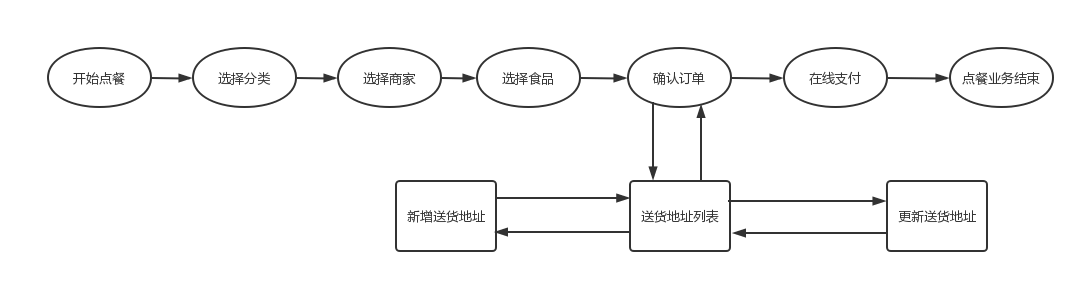
\includegraphics[scale=0.45]{figures/flowchart.png}
    \caption{业务流程图}
\end{figure}